% Revision 4 -- additions to Section IV/V (evaluation setup). Insert after the existing scenario
% table; the S1-S11 definitions are unchanged.

\subsection{Additional attack scenarios}\label{sec:scenarios}
Three scenarios exercise the generalised model of Sec.~\ref{sec:formulation}:
\begin{itemize}
\item \textbf{S12 / S13, multi-link.} Two (S12) or three (S13) target links are attacked at
  once, each by 3 flows of 30\,Mbps (the S11 overload, per link) for 120\,s, with two legitimate
  flows per target. Targets are the most-used fastest non-bridge links under static routing that
  share no switch with an earlier target.
\item \textbf{S14, adaptive rolling attacker.} The S11 budget (3 flows $\times$ 30\,Mbps, 120\,s),
  but every $\Delta_a=10$\,s the attacker observes the victims' current routes and re-aims at the
  link that most victim flows now share. It keeps flows that already cross that link and replaces
  the others with flows from fresh host pairs, chosen so that the \emph{defence's own} routing of a
  new flow (static, ECMP hash, $k$-path split, \dots) puts the largest share of the flow on the link.
  This is the rolling behaviour of Crossfire~\cite{kang2013crossfire} with a routing-aware
  attacker, i.e.\ the strongest attacker the threat model allows.
\end{itemize}
S12--S14 are evaluated in simulation only (Sec.~\ref{sec:sim}).
Table~\ref{tab:scenario_space} places every scenario in the scenario space of
Sec.~\ref{sec:formulation}, together with the ranges from which the randomised sweep of
Sec.~\ref{sec:sweep} draws 2{,}000 further instances.
% Revision 4 -- the hand-made scenarios as points of the scenario space (Sec. III-C), and the ranges the
% randomised sweep samples (sim/generic.py). alpha = target's offered load / capacity during the attack
% (legitimate 20 Mbps included), as in the measured-load checks of the emulation.
\begin{table}[t]\centering\scriptsize
\caption{Scenarios as points of the space $\omega=(G,c,\mathbf{r}^L,\mathcal{A},B_a,T_a,\pi_a)$ and the
ranges sampled by the randomised sweep.}\label{tab:scenario_space}
\setlength{\tabcolsep}{2.5pt}
\begin{tabular}{@{}lccccl@{}}
\toprule
 & topologies & $|T|$ & bots/target & $\alpha$ & behaviour $\pi_a$\\
\midrule
S1 & 4 & 0 & 0 & 0.2 & none\\
S2--S5 & 4 & 1 & 1--5 & 0.5--0.95 & constant\\
S6, S11 & 4 & 1 & 3 & 1.1 & constant, 600 / 120\,s\\
S7 & 4 & 1 & 3 & 0.85 / 0.65 & pulse, $P=8$\,s, $\delta=\tfrac12$\\
S8 & 4 & 1 & 3 & 0.9 & bursts of 8\,s every 31\,s\\
S9 & 4 & 1 & 3 & 0.9 & constant, detours pre-loaded to 0.79\\
S10 & 4 & 1 & 3 & as S7--S9 & S7--S9, randomised $N$, $T_c$\\
S12, S13 & 4 & 2, 3 & 3 & 1.1 & constant\\
S14 & 4 & 1 (moving) & 3 & 1.1 & rolling, $\Delta=10$\,s\\
SB & 4 & 0 & 0 & 0.9 in bursts & legitimate bursts only\\
\midrule
Sweep & 8 real + Waxman, BA & 1--3 & 1--5 & U[0.9, 1.6] & constant, pulse ($P\in\{4,8\}$,\\
 & (15--40 nodes) & & & & $\delta\in\{\tfrac13,\tfrac12,\tfrac23\}$), timed, rolling\\
 & \multicolumn{5}{l}{legitimate demand: gravity model, 10--60 flows, base load U[0.2, 0.6]}\\
\bottomrule
\end{tabular}
\end{table}


\subsection{Additional baselines}\label{sec:baselines}
Besides static shortest-path routing, static ECMP~\cite{rfc2992} and simple reactive rerouting, three
baselines represent multipath routing and optimal traffic engineering:
\begin{itemize}
\item \textbf{$k$-path multipath ($k$-MP)}: every flow is split equally over its $k=3$
  lowest-latency paths within the hop limit and never moved (oblivious, traffic-unaware spreading).
\item \textbf{TE-LP}: whenever any link is above $\theta$, the controller solves the min-max-utilisation
  LP~(\ref{eq:lp}) (HiGHS) over the $K=6$ lowest-latency paths of every active flow, with the
  measured rates of \emph{all} flows, and installs the fractional split. Ties are broken towards
  the current split and shorter paths so that equal-optimum solutions do not churn. It reacts on
  the first poll above $\theta$ (no trend detector) and splits single flows, which needs weighted
  select groups: it is an idealised TE upper bound in the spirit of
  SWAN/B4~\cite{hong2013swan,jain2013b4}, not a deployable equal of ResilientSDN.
\item \textbf{TE-$\Phi$}: the same LP with the objective of Eq.~(\ref{eq:objective}) instead of the
  maximum: minimise $\sum_e s_e$ with $s_e\ge u_e-\theta$, $s_e\ge0$ (the maximum utilisation only
  breaks ties), i.e.\ the LP relaxation of our own per-interval problem. We added it after observing
  that min-max TE is degenerate on G\'EANT: in 12 of 30 S11 runs a 5\,Mbps background flow on a
  1.55\,Mbps link (no detour among its candidate paths) fixes $U^\star=3.23$ whatever the routing, so
  every split that keeps the attacked link below 3.23 is optimal and the LP never relieves it.
\end{itemize}
\textbf{ResilientSDN-v2} is Algorithm~\ref{alg:rsdn} with the two extensions turned on (severity
order, fallback) and the bottleneck form of~(\ref{eq:dpp}) with $V_0=0.1$; ResilientSDN without
suffix is the published configuration. \textbf{ResilientSDN-v3} adds a duty-cycle trigger to v2: a
link that is above $\theta$ now also counts as congested if it was above $\theta$ in at least half of the
last $M=6$ polls (12\,s). It targets the pulse attack S7, which alternates 85\,\% and 65\,\% load every
4\,s and so is never above $\theta$ for $N=3$ consecutive polls; the legitimate bursts of ablation D
(above $\theta$ in at most 2 of 6 polls) must not trigger it, which we test with the scenario
\textbf{SB} (S1 traffic plus those bursts).

\subsection{Flow-level simulation}\label{sec:sim}
The Mininet testbed takes about 90\,s per run (630\,s for S6), which limits it to five runs per
cell and to the scenarios already reported. To add seeds, scenarios, TCP traffic and the LP baseline
we built a flow-level simulator (\texttt{sim/}) that runs the \emph{same decision code} as the Ryu
controller (Algorithm~\ref{alg:rsdn} lives in one module imported by both) and the same traffic
planner, so targets, host pairs and rates are identical to the emulation for the same seed.
The model advances in 1\,s steps:
UDP flows are inelastic and an overloaded link drops the excess in proportion to arriving rates
(with upstream drops propagated downstream);
TCP flows are elastic 5\,MB transfers (access cap 20\,Mbps, 1\,s think time between transfers) that
share what UDP leaves by max-min fairness~\cite{bertsekas1992data}, with a floor of 5\,\% of a
saturated link (TCP is not modelled as starving completely under drop-tail).
The controller sees what OpenFlow counters would report: carried link load ($\le c_e$) and the
ingress rate of every flow, averaged over the 2\,s polling interval. Not modelled: queueing delay,
TCP dynamics below the 1\,s step (slow start, reordering after a path change), packet-level
burstiness and control-plane latency.
\textbf{Validation.} On the \valCells\ (topology, scenario) cells and \valPoints\ (cell, system)
points that both the simulator and an earlier emulation campaign (1~October 2026, 390 runs, same
traffic protocol; its summary table is in \texttt{paper\_rev4/data}) cover, the Spearman correlation
of seconds above threshold is \valRhoTime\ (loss: \valRhoLoss), and the simulator ranks the three
systems the same way as the emulation in \valAgree\ of \valCells\ cells
(Fig.~\ref{fig:validation}). The main systematic difference is that the simulator relieves a link
about 2\,s earlier (no rule-installation delay). We therefore use the simulator for relative
comparisons across many seeds and scenarios, and the emulation for absolute values.

\begin{figure}[t]\centering
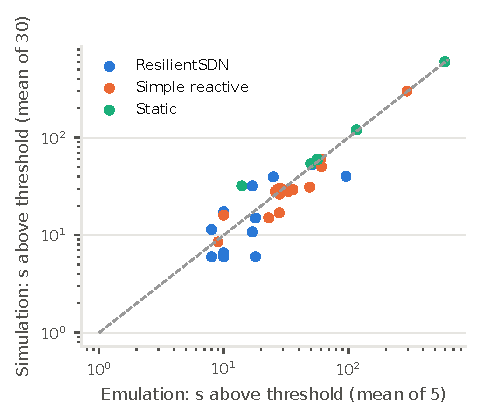
\includegraphics[width=\columnwidth]{figures/validation}
\caption{Simulation against emulation: mean seconds above $\theta$ per (topology, scenario, system).
Dashed: identity.}\label{fig:validation}
\end{figure}

\subsection{Seeds and statistics}\label{sec:stats}
Simulation cells use 30 seeds (\simRunsUDP\ UDP runs, \simRunsTCP\ TCP runs, \simRunsEcmp\ runs
with an ECMP-aware attacker); emulation cells keep 5. Run $r$ of a cell gives every system the same
traffic, so comparisons are \emph{paired}: for each cell, metric and system we report the mean
per-seed difference to ResilientSDN with a 95\,\% percentile-bootstrap CI (10\,000 resamples), the
two-sided Wilcoxon signed-rank test~\cite{wilcoxon1945}, the matched-pairs rank-biserial
correlation as effect size~\cite{kerby2014rankbiserial}, and Holm-Bonferroni
correction~\cite{holm1979} over all tests of a table. This replaces the earlier unpaired,
uncorrected Welch tests (\texttt{evaluation/paired\_stats.py}).
